Cet exercice s'intéresse à la croissance d'une personne appelée Juliette. Sa croissance est modélisée par la fonction $f$, représentée ci-dessous.

La \textbf{vitesse de croissance} de Juliette (en cm par an) à une date donnée $t$ est égale au \textbf{nombre dérivé} $\boldsymbol{f'(t)}$.

On a également représenté trois tangentes à la courbe représentative de $f$ : celles aux points A, B et C.

\begin{center}
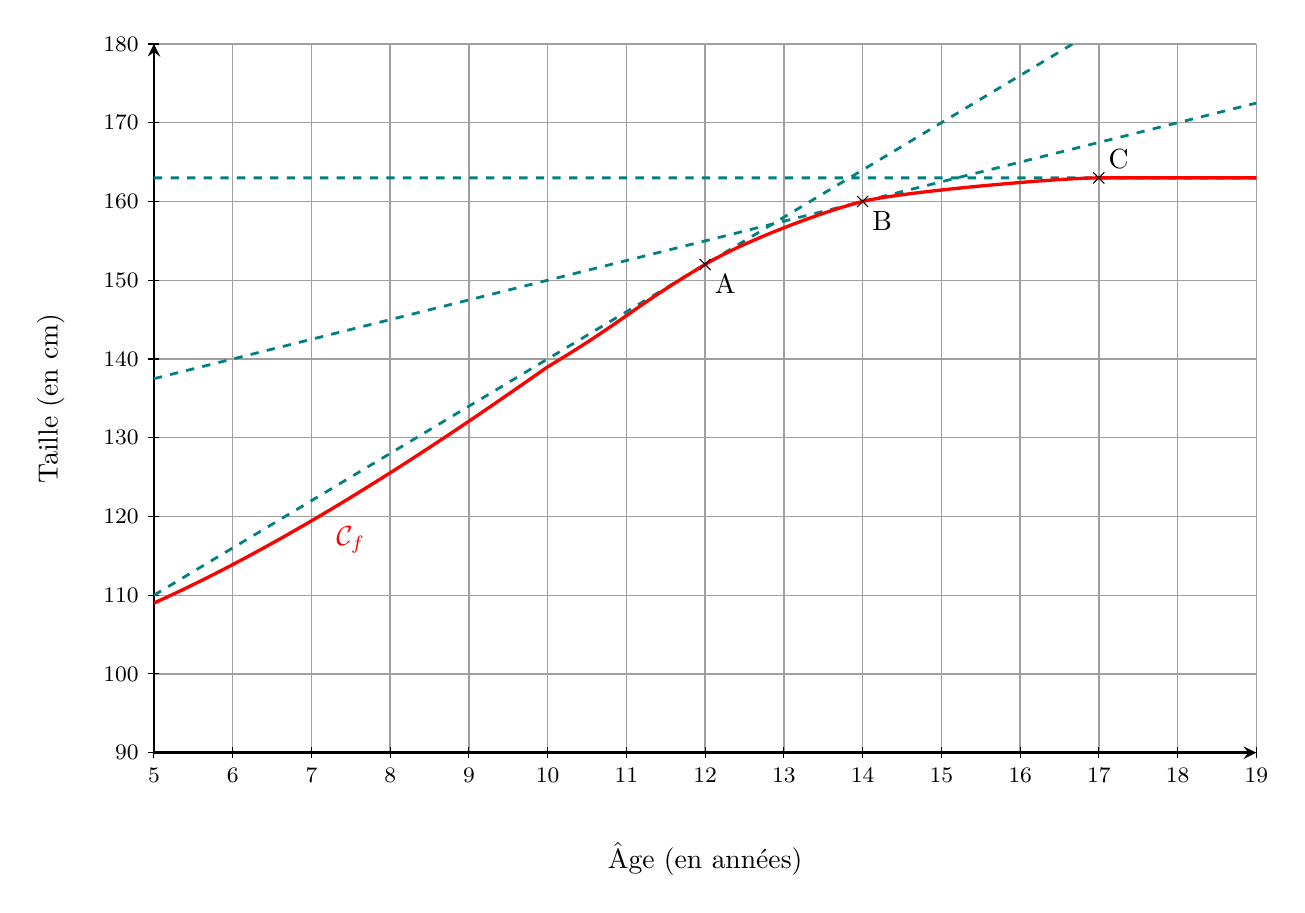
\begin{tikzpicture}[x = 1cm, y=1mm]
	\draw [color = gray!75, line width = 0.5pt, xstep=1, ystep = 10] (5,90) grid (19,180);
	\draw[<->, line width=1pt,>=stealth] (19,90)--(5,90)node[pos=0.5, below=1cm]{Âge (en années)} -- (5,180) node[pos=0.5,sloped,above=1cm]{Taille (en cm)};
	\foreach \x in {5,...,19}
	\draw[shift={(\x,90)},color=black] (0pt,2pt) -- (0pt,-2pt) node[below, fill = white] {\footnotesize $\np{\x}$};
	\foreach \y in {90,100,...,180}
	\draw[shift={(5,\y)},color=black] (2pt,0pt) -- (-2pt,0pt) node[left, fill = white] {\footnotesize $\np{\y}$};
	\clip (5,90) rectangle (19,180);
	\draw[dashed, line width=1pt,teal] (5,110)--(17,182)
		(5,137.5)--(19,172.5)
		(5,163)--(19,163) ;
	\draw[line width=1.2pt,color=red,smooth]
	(5,109) ..controls (7,118) and (9,132)..
	(10,139)..controls (11,145) and (11,146)..
	(12,152)..controls (12.5,155) and (13.5,158.75)..
	(14,160)..controls (14.5,161.25) and (16.5,163)..
	(17,163) -- (19,163);
	\node[red] at (7.5,117) {$\mathcal{C}_f$};
	\foreach \nom/\coord/\pos in {A/{(12,152)}/{below right},B/{(14,160)}/{below right},C/{(17,163)}/{above right}}
		{\draw[shift={\coord}] (-2pt,-2pt)--(2pt,2pt) (-2pt,2pt)--(2pt,-2pt) (0,0) node[\pos]{\nom} ;}
\end{tikzpicture}
\end{center}

On répondra aux questions suivantes avec la précision permise par le graphique :

	\begin{enumerate}
		\item Estimer la taille de Juliette le jour de ses 14 ans.

		\item À quel âge Juliette grandissait-elle le plus vite, à 12 ans ou à 14 ans ? \emph{Justifier.}

		\item Pourquoi peut-on considérer que Juliette a terminé sa croissance à 17 ans ?

		\item Estimer la taille adulte de Juliette.
	\end{enumerate}
